% !TEX encoding = IsoLatin2  % notwendige Zeile für Mac-Benutzer (muss als Kommentar stehen); Windows-Benutzer können die Zeile löschen.

% LaTeX-Vorlage Version 3.1,  Juli 2011
% erstellt von Dr. Andreas Drauschke (andreas.drauschke@technikum-wien.at) und Dr. Susanne Teschl (susanne.teschl@technikum-wien.at)
% geringfügig adaptiert von Harald Stockinger (harald.stockinger@technikum-wien.at)

 
\documentclass[a4paper,bibtotoc,oneside]{scrbook} 
% Für kurze Arbeiten wäre auch die Dokumentklasse "scrartcl" ausreichend. In diesem Fall ist "section" die höchste Ebene ("chapter" gibt es dann nicht).
% \documentclass[a4paper,bibtotoc,oneside]{scrartcl}

%\usepackage{cclicenses}

% verlinkte Querverweise im pdf
\usepackage{hyperref}

% deutsche Anpassungen
\usepackage[utf8]{inputenc}
\usepackage[T1]{fontenc}
\usepackage[ngerman]{babel}


% mathematische Symbole
\usepackage{amsmath,amssymb,amsfonts,amstext}

% Kopfzeilen frei gestaltbar
\usepackage{fancyhdr}
\lfoot[\fancyplain{}{}]{\fancyplain{}{}}
\rfoot[\fancyplain{}{}]{\fancyplain{}{}}
\cfoot[\fancyplain{}{\footnotesize\thepage}]{\fancyplain{}{\footnotesize\thepage}}
\lhead[\fancyplain{}{\footnotesize\nouppercase\leftmark}]{\fancyplain{}{}}
\chead{}
\rhead[\fancyplain{}{}]{\fancyplain{}{\footnotesize\nouppercase\sc\leftmark}} 

% Farben im Dokument möglich
\usepackage{color}

% Schriftart Helvetica
\usepackage{helvet}
\renewcommand{\familydefault}{cmss} 

% Graphiken einbinden: hier für pdflatex
\usepackage[pdftex]{graphicx}

\usepackage{array}

% Höhe und Breite des Textkörpers etwas grösser definieren
\setlength{\textheight}{225mm}
\setlength{\textwidth}{1.05\textwidth}

% weniger Warnungen wegen überfüllter Boxen
\tolerance = 9999
\sloppy

% Anpassung einiger überschriften 
\renewcommand\figurename{Abbildung}
\renewcommand\tablename{Tabelle}

\begin{document}

% Kopf- und Fusszeilen initiieren
\pagestyle{fancy}
\pagenumbering{Alph}

% Deckblatt:
\thispagestyle{empty}
\begin{picture}(0,0)
\color{white}\sffamily
\put(-101,-749){
\includegraphics[width=1.002\paperwidth, height=\paperheight]{BM_2011.pdf}}
\put(220,-670){
\includegraphics[width=0.5\textwidth]{FHTW_Logo_4c.pdf}}
\put(-30, -20){\bfseries\huge BACHELORARBEIT}
% Titel des Studienganges einfügen:
\put(-30,-50){\Large im Studiengang Bachelor Informatik}
% Titel der Arbeit einfügen:
% Die Minipage wird gesetzt, damit auch mehrzeilige Titel möglich werden.
\put(-32,-150){
\begin{minipage}{14cm}
\bfseries\huge Software-Test von Web-Applikationen
\end{minipage}
}
% Name der Autorin/des Autors eingeben:
\put(-30,-250){\large Ausgeführt von: Bernhard Posselt}
% Personenkennzeichen der Autorin/des Autors eingeben:
\put(-30,-270){\large Personenkennzeichen: 1010257029}
% Name der Begutachterin/des Begutachters eingeben:
\put(-30,-310){\large Begutachter: MSc Benedikt Salzbrunn}
\put(-30,-350){\large Wien, \today} % das Datum des letzten Kompilierens wird automatisch eingesetzt
\color{black}
\end{picture}

\newpage


\section*{Eidesstattliche Erklärung}\thispagestyle{empty}
\glqq Ich erkläre hiermit an Eides statt, dass ich die vorliegende Arbeit selbständig angefertigt habe. 
Die aus fremden Quellen direkt oder indirekt übernommenen Gedanken sind als solche kenntlich gemacht. 
Die Arbeit wurde bisher weder in gleicher noch in ähnlicher Form einer anderen Prüfungsbehörde vorgelegt
und auch noch nicht veröffentlicht. Ich versichere, dass die abgegebene Version jener im Uploadtool entspricht.\grqq\\[5\baselineskip]
\rule{5cm}{0.2pt}\hfill\rule{5cm}{0.2pt}\\
\phantom{Datum }Ort, Datum\hfill Unterschrift\hspace{15mm}

\newpage


\section*{Kurzfassung}\thispagestyle{empty}
Die Durchführung und Erstellen von automatisierten Tests für Web-Applikationen unterscheidet sich von klassischen Applikationen. Aufgrund der komplexeren Infrastruktur und Modularisierung werden zusätzliche Testfälle und Strategien benötigt um Web-Applikationen ausreichend abzudecken und eine fortwährende Qualität zu gewährleisten. Diese Arbeit soll Möglichkeiten für den Test von Web-Applikationen aufzeigen.

\vfill
\paragraph*{Schlagwörter:} Webapplikationen, automatisierte Tests, Webtest


\newpage

\section*{Abstract}\thispagestyle{empty}
Creation and execution of automatic web application tests is different from tests of classic applications. A more complex infrastructure and modularisation require additional testcases and strategies to guarantee a good enough test coverage which in return ensures constant quality. This thesis highlights various possibilities to test web applications.

\vfill
\paragraph*{Keywords:} web applications, automatic tests, webtest
\newpage

%\section*{Danksagung}
%\thispagestyle{empty}
%Text Text Text Text Text Text Text Text Text Text Text Text Text Text Text Text
%\newpage

\tableofcontents\thispagestyle{empty}
\newpage

\pagenumbering{arabic}
\setcounter{page}{1}

% Falls die Kapitelüberschriften zu lang für die Kopfzeile oder das Inhaltsverzeichnis sind, so erzielt man
% dort Kurzformen der Kapitelbezeichnungen mittels:
% \chapter[Kurzform]{Lange überschrift}
\chapter{Einführung}
Durch die zunehmende Verbreitung von Smartphones und anderen mobilen Geräten erfährt der Markt für Software-Applikationen eine zunehmende Fragmentierung \cite{smartphone}[S. 1]. Viele dieser Plattformen erfordern das Erlernen von unterschiedlichen Programmiersprachen, Toolkits und Betriebssystemen \cite{android}\cite{ios}. Will ein/eine Software-EntwicklerIn eine Applikation plattformübergreifend anbieten, erfordert dies daher einen höheren Zeit- und Kostenaufwand.

Da viele dieser Mobilgeräte über einen Web-Browser verfügen, wird das Web als Applikationsplattform immer attraktiver und bestimmte Software-Tools wie PhoneGap \cite{phonegap} erlauben dem/der EntwicklerIn sogar eine plattformübergreifende Mobil-Applikationen auf Basis von Web-Technoligien zu erstellen, welche sich nahtlos in das System integrieren. Durch die Verwendung unterschiedlicher Web-Browser erhöht sich jedoch auch die Fehler-Rate der Applikation. 

\section{Fehler in Software-Applikationen}
Keine Applikation ist fehlerfrei\cite{empiric_invest}[S. 9]. Diese Fehler  führen nicht nur zu unzufriedenen Kunden, sondern auch zu hohen Kosten: \glqq Im Jahr 2000 wurde in den USA ein Schaden durch Softwarefehler in der Auto- und Flugzeugindustrie von 1,8 Milliarden US-Dollar errechnet. Dies entspricht ca. 16 \% des Softwareumsatzes\grqq\\\cite{betrieb}[S. 15]

Die Fehler-Rate wird auf ungefähr 3 pro 1.000 Zeilen geschätzt, was bei einer aufwendigeren Applikation mit 100 Millionen Zeilen Quellcode eine durchschnittliche Anzahl von von 300.000 Fehlern ergibt \cite{eval_regression}[S. 10]. 

Je früher diese Fehler entdeckt werden, desto kostengünstiger können diese beseitigt werden \cite{betrieb}[S. 17]. Daher ist es wichtig, möglichst früh mit dem Testen zu beginnen und es in den Software-Entwicklungsprozess zu integrieren \cite{betrieb}[S. 16]. 

\section{Grenzen von Software-Tests}
Das Vorhandensein von Tests kann jedoch niemals eine komplett fehlerfreie Software garantieren, nur eine Abwesenheit von bestimmten Fehlern kann garantiert werden, nämlich jenen, die explizit mit Tests abgedeckt werden. \cite{eval_regression}[S. 12]

Außerdem ist es nicht erstrebenswert, die ganze Applikation mit Tests abzudecken, da dies zu zu hohen Entwicklungskosten führen kann. Idealerweise werden daher nur jene kritischen Fälle mit Tests abgedeckt, deren Fehlerkosten die Kosten für die Erstellung der Tests übertreffen. \cite{eval_regression}[S. 12]

Die implementierten Testfälle müssen auch regelmäßig gewartet und aktualisiert werden, um ihre Effektivität zu gewährleisten, denn diese nimmt auf Dauer ab. Es ensteht eine sogenannte \glqq Testresistenz\grqq\\\cite{eval_regression}[S. 12], die daraus resultiert, dass die bestehenden Tests nur bekannte Fehlerfälle abdecken und neue mögliche Fehlerfälle nicht berücksichtigen. \cite{eval_regression}[S. 12-13]

\section{Testen im Projektmanagement}
Tests können jedoch nicht nur dazu verwendet werden, um Fehler in der Applikation zu finden, sondern auch um einen Überblick über den derzeitigen Stand der Implementation zu gewinnen: Sie geben dem/der EntwicklerIn und ProjektmanagerIn ein direktes Feedback über bereits korrekt implementierte Teile der Software-Spezifikation. Auch Milestones können durch Tests definiert werden. \cite{test_auto}[S. 2]

\section{Vorteile von automatisierten Tests}
Da die vorhandenen Tests durch die Einbindung in den Entwicklungsprozess öfters durchgeführt werden müssen, kann sich durch das manuelle Testen der immer gleichen Tests schnell eine gewisse Eintönigkeit einstellen. Das wiederum kann unter anderem dazu führen, dass Tester bestimmte Tests nicht korrekt oder ineffizient ausführen. 

Dieses Problem kann durch eine Automatisierung des Testprozesses gelöst werden. Die Automatisierung erlaubt zudem bei zukünftigen Testdurchläufen eine Reduzierung auf ein Minimum des ursprünglichen Zeitaufwandes. Daher sollte versucht werden, möglichst viele dieser Tests zu automatisieren. \cite{test_auto}[S. 22-23]


%\cite{test_large_systems}[S. 10]


%test ist mehr als simples aufnehmen und abspielen von inputs: ist redundant und eintönig, muss automatisiert werden muss geplant werden und auch generisch sein ansonsten braucht wartung der test skripte mehr aufwand und reibereien mit kollegen wenn sie etwas ändern
%automatisiertes monkey testing findet nur absturz bugs aber keine funktionalen bugs 

%Vorbereitung ca doppelt so hoch für automatisierten test reduziert sich aber auf minimum wenn mehrmals 

%Tests sind über nahct möglich brauchen aber höheren wissensstand zum erstellen\cite{eval_automat_webapp_test}[S. 37]

\section{Aufbau}


\chapter{Unterschiede zu klassischer Software}
Im Gegensatz zu klassischen Desktop- oder Mobil-Applikationen bestehen Web-Applikationen wegen ihrer Client-Server-Architektur immer aus mehreren Modulen, die meist über ein Netzwerk miteinander verbunden sind, beispielsweise: 

\begin{itemize}
\item Datenbank-Server
\item Web-Server
\item Applikations-Server
\item Authentifizierungs-Server
\item Web-Browser
\end{itemize}

Durch diesen modularen Aufbau ist es besonders schwer einen Fehler zu lokalisieren. Ein Fehler kann z.B. durch einen Fehler im Quellcode des Applikations-Servers oder durch ein Netzwerkproblem entstanden sein. \cite{testing_apps_on_web}[Foreword]

Außerdem gibt es eine größere Vielfalt an Plattformen, auf welchen Web-Applikationen ausgeführt wird: Auf der Serverseite sind diese Plattformen noch vom/von der BetreiberIn festlegbar, sprich welches Betriebssystem und welche Datenbank eingesetzt wird, auf der Clientseite ist dies aber schon nicht mehr möglich. Die BesucherInnen der Webseite verwenden verschiedene Web-Browser auf verschiedenen Betriebssystemen, welche beide in unterschiedlichen Versionen vorliegen können. Auch können unterschiedliche Plugins und Fonts in unterschiedlichen Versionen installiert sein. \cite{testing_apps_on_web}[Foreword]

Zudem verlagert sich auch immer mehr Applikations-Logik von der Server- auf die Clientseite\cite{testing_apps_on_web}[S. 13]. Durch das Verwenden von \emph{Events}, welche unter anderem durch BenutzerInnen-Eingaben ausgelöst werden können, stellt clientseitiger Code eine größere Herausforderung für den/die TesterIn dar als Serverseitiger: Events können in unterschiedlicher Reihenfolge und Kombination auftreten, manche Aktionen lösen sogar mehrere Events aus. \cite{testing_apps_on_web}[S. 18]

Eine weitere Herausforderung stellt das Session Modell von Web-Applikationen dar: viele Web-Applikationen verwenden nur eine Session pro NutzerIn, erlauben aber mehrere gleichzeitige Logins. Werden mehrere Instanzen der Applikation gestartet - z.B. loggt sich der/die NutzerIn auf dem Mobiltelefon und dem Laptop auf der Webseite ein - kann dies zu Synchronisationsproblemen zwischen den einzelnen Instanzen führen: Wird in einer Instanz ein Eintrag gelöscht, kann dieser durch eine fehlerhafte Synchronisation in einer andere Instanz immer noch existieren und in weiterer Folge zu Fehlern führen. \cite{testing_apps_on_web}[S. 20]

Diese Vielfalt an verschiedenen möglichen Konfigurationen und Herausforderungen erfordert eine neue Herangehensweise an das Thema Software-Test: Die bestehenden Techniken sind \glqq zwar auch notwendig, aber nicht ausreichend, um die Qualität der Applikation sicherzustellen\grqq\ \cite{eval_automat_webapp_test}[S. 18]



%\chapter{Testplan}
%was und wo testen (hardware/software)
%wann 
%wer

%testinputs identifizieren (alles was validiert werden muss und von was die sw abhängt) auch wichtig für änderungen
%dann testplan: ziele + sinn der tests und strategien wie man es umsetzt
%der beinhaltet testfälle
%dann spezifizieren wann jeder testfall funktionieren muss sprich bei welchem milestone und config spezifizieren \cite{test_auto}[S. 3-4]



%Planning + Documentation, testplan\cite{testing_apps_on_web}[S. 34]
%\cite{test_auto}[S. 3]
%\chapter{Unit Test}
%\chapter{Integration Test}
%\cite{process_oop}[S. 30]
%\chapter{Acceptance Test}
%
%\cite{test_auto}[S. 11]
%
%Development acceptance tests:
% data driven \cite{test_auto}[S. 24]
% * Release acceptance tests (smoke tests): mainstream data + mainstream funktionen \cite{testing_apps_on_web}[S. 36]
% * Functional acceptance simple test: each dev release to test accessibility of key features on minimum configuration, no full functionality test (file saving example) \cite{testing_apps_on_web}[S. 37-38]

%Deployment acceptance tests:
%Full installation + configurations
% * Task-Oriented Functional Test: Features test (gherkin) against requirements, specs + design docs \cite{testing_apps_on_web}[S. 42]
% * Forced Error Test: testing for failures 
% * boundary test: test extreme inputs
% * system level test: test whole application \cite{testing_apps_on_web}[S. 43]
% * real world user level test: echte leute testen um fehler zu finden die man sonst übersieht
% * exploratory test: überlegen wo es probleme geben könnte und dort testen
% * stress test: limited resource conditions (memory, diskspace, network bandwidth)
% * Performance tests: testen wieviel das system verträgt
% * Regression tests: für bugs die schonmal aufgetreten sind \cite{testing_apps_on_web}[S. 44]
% * Compability + config tests: testen auf unterschiedlichen platformen
% * documentation test: testen von zb shortcuts \cite{testing_apps_on_web}[S. 45]
% * install uninstall test
% * UX tests
% * External beta tests \cite{testing_apps_on_web}[S. 46]
% * Secuirty tests
% * Unit tests

%\section[Erster Abschnitt]{überschrift des ersten Abschnitts}



%\subsection[Erster Unterabschnitt]{überschrift des ersten Unterabschnitts}



%\subsubsection[Erster Unter-Unterabschnitt]{Und noch eine Ebene tiefer} 


%\\[2\baselineskip]
%Hier wird auf Abbildung~\ref{Abb1} verwiesen. 
%\begin{figure}[htbp]
%\centering
%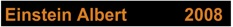
\includegraphics[width=75mm]{Buchruecken}
%\caption[Beschriftung eines Buchrückens.]{Beispiel für die Beschriftung eines
%Buchrückens.}\label{Abb1}
%\end{figure}
%%Tabelle~\ref{Tab1} ist ein Beispiel dafür, wie eine Tabelle aussehen könnte.
%\begin{table}[htbp]
%\centering
%\begin{tabular}{ | c | c | c | }\hline
%{\bf Datum} & {\bf Thema} & {\bf Raum}\\ \hline
%\hline
%20. 08. 2008 & Graphentheorie & HS 3.13\\ \hline
%01. 10. 2008 & Biomathematik & HS 1.05\\ \hline
%\end{tabular}
%\caption[Semesterplan "`Angewandte Mathematik"'.]{Beispiel für einen
%Semesterplan "`Angewandte Mathematik"'.}\label{Tab1}
%\end{table}

%\noindent
%Nun ein Beispiel für eine abgesetzte Formel:
%\begin{equation}
%x =  - \frac{p}{2} \pm \sqrt{\left(\frac{p}{2}\right)^2 - q}.
%\end{equation}
%Und eine mehrzeilige Formel:
%\begin{eqnarray}
%f(t)&=& t^2 \label{For1},\\
%g(t) &=& t-1.
%\end{eqnarray}
%Hier wird auf die Formel (\ref{For1}) verwiesen. \\

%\noindent
%So kann zum Beispiel ein \glqq Source-Code\grqq\  angegeben werden: 
%\begin{verbatim}
%for (i=1; i < 10; i++) {...} 
%\end{verbatim}

%\noindent
%Hier ist ein Hyperlink auf die  \href{http://www.technikum-wien.at}{Homepage}
%der FH Technikum Wien. Email-Adressen können so verlinkt werden:
%\href{mailto:homer.simpson@springfield.com}{\texttt{
%homer.simpson@springfield.com}}\\

%\noindent
%In der Bibliothek der Fachhochschule Technikum Wien gibt es verschiedene
%einführende Bücher zum Thema \glqq \LaTeX \grqq, zum Beispiel \cite{kop05},
%\cite{wil06} oder \cite{mgb+05d} (deutsche Version) bzw. \cite{mgb+04e}
%(englische Version). Empfehlenswerte Skripten für \LaTeX-Einsteiger sind z.B.
%\cite{mj00} und \cite{mj95}. Sie sind frei im Internet verfügbar.



% Literaturverzeichnis
% Das Literaturverzeichnis kann auch nach einem allfälligen Anhang positiioniert werden (siehe "`Leitfaden für Bachelor- und Diplomarbeiten"', Version 2.0, Abschnitt 2.9).

% Möglichkeit 1: Erzeugung des Literaturverzeichnisses mit BibTeX:
% Die Quellen sind in der Datei *.bib (hier Literatur.bib) einzugeben. Danach muss diese Vorlage einmal geTeXt werden, dann BibTeX angewendet werden und 
% anschliessend nochmals zweimal geTeXt werden.
% Im Text erfolgt die Zitierung mit dem Anker-Schlüsselwort, z.B. \cite{kop05}.
\bibliographystyle{IEEEtran}
\bibliography{Literatur}

% Möglichkeit 2: Erzeugung eines Literaturverzeichnisses ohne BibTeX:
%\begin{thebibliography}{99}
%\bibitem[kop05]{kop05}
%H.~Kopka, {\em LaTeX, Band 1: Einführung}, Pearson Studium, München, 3.~Auflage, 2005.
%\bibitem[knu98]{knu98}
%F.~Mittelbach, M.~Goossens, J.~Braams, D.~Carlisle, and Ch. Rowley, {\em The LaTeX Companion}, 
%Addison-Wesley, 2nd edition, 2004.
%\end{thebibliography}

% Abbildungsverzeichnis
\listoffigures
\addcontentsline{toc}{chapter}{Abbildungsverzeichnis} % fügt den Eintrag äbbildungsverzeichnis" im Inhaltsverzeichnis hinzu
\newpage

% Tabellenverzeichnis
%\listoftables 
%\addcontentsline{toc}{chapter}{Tabellenverzeichnis} % fügt den Eintrag
%"Tabellenverzeichnis" im Inhaltsverzeichnis hinzu
%\newpage

% Abkürzungsverzeichnis
% Bei Verwendung der Dokumentklasse "scrartcl" ist der Befehlt \addchap{Abkürzungsverzeichnis} durch 
% \addsec{Abkürzungsverzeichnis} zu ersetzen
\addchap{Abkürzungsverzeichnis}
\hspace{-17mm}\begin{tabular}{>{\raggedleft}p{0.2\linewidth} p{0.75\linewidth} p{0.1\linewidth}}

% www & World Wide Web\\

\end{tabular}

% Anhänge
%\begin{appendix}
%\chapter[Erster Anhang]{überschrift des ersten Anhangs}

%Text Text Text Text Text Text Text Text Text Text Text Text Text Text Text Text
%\end{appendix}

\end{document}
